\documentclass[a4paper, 11pt]{article}
\usepackage{graphicx}
\usepackage{amsmath}
\usepackage[pdftex]{hyperref}
\usepackage{algorithm}
\usepackage{algorithmic}
\usepackage{epstopdf}
\usepackage{subcaption}

% Lengths and indenting
\setlength{\textwidth}{16.5cm}
\setlength{\marginparwidth}{1.5cm}
\setlength{\parindent}{0cm}
\setlength{\parskip}{0.15cm}
\setlength{\textheight}{22cm}
\setlength{\oddsidemargin}{0cm}
\setlength{\evensidemargin}{\oddsidemargin}
\setlength{\topmargin}{0cm}
\setlength{\headheight}{0cm}
\setlength{\headsep}{0cm}

\renewcommand{\familydefault}{\sfdefault}

\title{Data Mining: Learning from Large Data Sets - Spring Semester 2014 Projects}
\author{nivo@student.ethz.ch\\ ganzm@student.ethz.ch\\ rohrp@student.ethz.ch\\}
\date{\today}

\begin{document}
\maketitle

\section{Approximate near-duplicate search using Locality Sensitive Hashing} 

This section explains the implementation of project 1. In this first project we
were supposed to find near-duplicate videos using Locality Sensitive Hashing.
The videos were given as a number of shingles that could be compared. The
implementation was done in Python to be used in combination with the hadoop
infrastructure. This means we implemented a mapper and a reducer that read from
stdin and write to stdout. In the following two sections we explain the
functionality of the mapper and the reducer each.

\subsection*{mapper.py}

The mapper creates a signature vector of a video. This signature
vector is afterwards subdivided into $b$ bands having $r$ elements that get
hashed. Each band and its hash are then emitted.

These are the steps in more detail:

\begin{enumerate} 

\item As \autoref{fig:func} shows, choosing $b=32$ and $r=8$ does not miss any true positives.

\begin{figure}
\centering
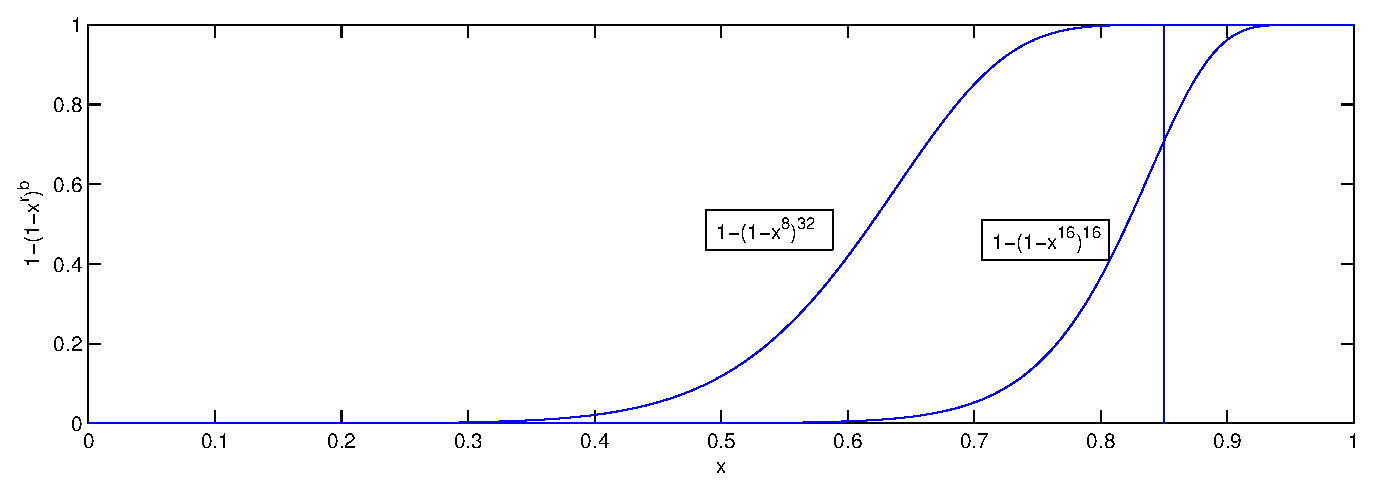
\includegraphics[scale=.5]{project1/func.eps}
\caption{$1-(1-x^r)^b$}\label{fig:func}
\end{figure}

\item We create $k = b \cdot r$ hashfunctions of the form $ a_px + b_p \mod c_p$
where $a_p=rand(0,999), b_p=rand(0,99999)$, $c_p=10000$ and $rand(x,y)$ is
random variable drawn from a uniform distribution between $x$ and $y$. These
hashfunctions are used to calculate the permutations used for min-hashing.

\item We create $r$ hashfunctions of the form $ a_bx + b_b \mod c_b$ where
$a_b=rand(0,999), b_b=rand(0,999)$, $c_b=1000$ and $rand(x,y)$ is random
variable drawn from a uniform distribution between $x$ and $y$. These
hashfunctions are used to calculate the band hashes before emitting.

\item The signature is then created according to \autoref{alg:signature}

\begin{algorithm}

\caption{Create signature}\label{alg:signature}

\begin{algorithmic} 

\STATE $signature = \infty$

\FORALL{shingle in shingles}

\FOR{i in range(k)}

\STATE{ $signature[i] =min ({a_p}_i \cdot shingle + {b_p}_i \mod c_p,
signature[i])$}

\ENDFOR

\ENDFOR

\end{algorithmic} \end{algorithm}


\item Calculate the band hash and emit the band hash and the band as key, and
the video with its corresponding shingles as value according to
\autoref{alg:emit}

\begin{algorithm}
\caption{Emit keys and values}\label{alg:emit}
\begin{algorithmic} 

\FOR{band in range(b)}

\STATE{ $vector = signature[band \cdot r : band \cdot r + r]$}

\STATE{ $band hash = \sum_{i=1}^{len(vector)}{ {a_b}_i\cdot vector[i] + {b_b}_i \mod c}$}

\STATE{ emit $key=[band hash, band]$ $value=[video\_id, shingles]$ }

\ENDFOR

\end{algorithmic} \end{algorithm}


\end{enumerate}


\subsection*{reducer.py}

The main task of the reducer is to get rid of the false positives by comparing
the reported similar videos using the jaccard distance:

\begin{enumerate}

\item gather all videos with the same key in a collection $duplicates$
\item emit similar videos like shown in \autoref{alg:reducer}


\begin{algorithm}
\caption{Emit similar videos}\label{alg:reducer}
\begin{algorithmic} 

\FOR{i=0 to len(duplicates)}

\FOR{j=i+1 to len(duplicates)}

\IF{$duplicates[i].video\_id < duplicates[j].video\_id$}

\STATE{ $shingles\_left = duplicates[i].shingles$}
\STATE{ $shingles\_right = duplicates[j].shingles$}

\STATE{ $distance = \frac{\left| shingles\_left \cap shingles\_right \right|}{\left| shingles\_left \cup shingles\_right \right|}$}

\IF{$distance > 0.85$}

\STATE{ emit duplicates[i].video\_id duplicates[j].video\_id }

\ENDIF

\ENDIF

\ENDFOR

\ENDFOR

\end{algorithmic} 
\end{algorithm}



\end{enumerate}


\section{Large-Scale Image Classification}

This section describes the implementation of project 2. The task was to
implement binary classification on a large number of images.

\subsection{mapper.py: Stochastic Gradient Descent}

For the mapper functionality we chose to implement the PEGASOS
\cite{shalev2011pegasos} algorithm discussed in the lecture. The trained normal
vector $w$ is emitted out of each mapper.


\subsection{Feature transformation}

To reduce the classification error, meaning having less falsely classified
images we implemented following transformations.

\subsubsection{Normalisation}


As a feature transformation we chose to normalize our data first. Based on the
training data both mean and variance was calculated. These two calculated
vectors were hard coded into the mapper function to apply the following
transformation to the data:

$$ x' = \phi(x) = { {x - \mu} \over \sigma} $$ 

This transformation indeed seems to make sense when looking at figure
\ref{fig:mean-var}. Both mean and variance are somewhat scattered.

\begin{figure}[H]
\centering
\begin{subfigure}{.4\textwidth}
  \centering
  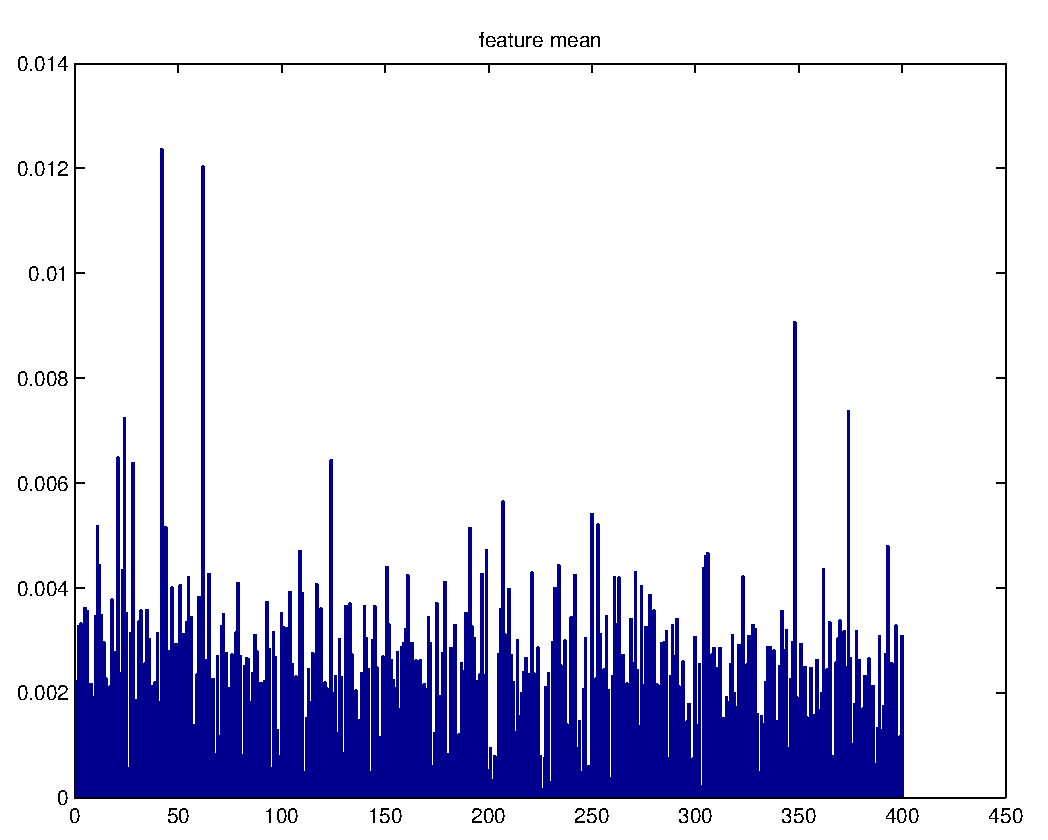
\includegraphics[scale=0.35]{project2/feature-mean.eps}
  \caption{Feature Mean}
  \label{fig:sub1}
\end{subfigure}%
\begin{subfigure}{.4\textwidth}
  \centering
  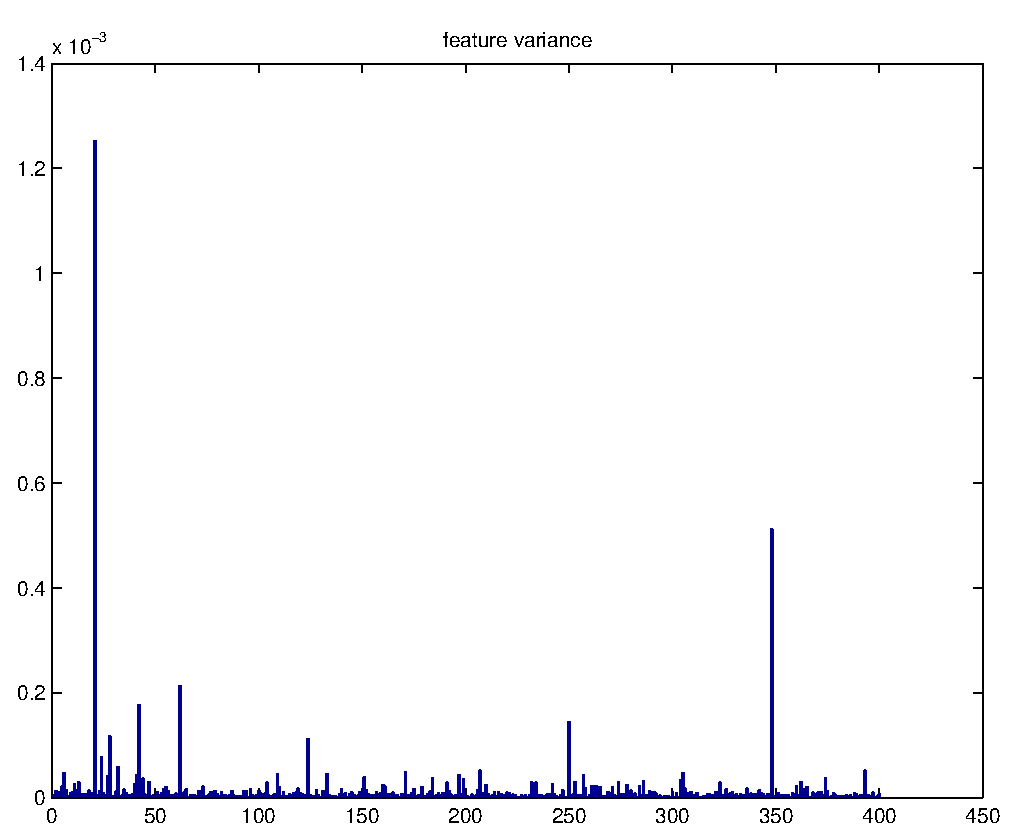
\includegraphics[scale=0.35]{project2/feature-variance.eps}
  \caption{Feature Variance}
  \label{fig:sub2}
\end{subfigure}
\caption{Mean and Variance of Feature Vectors}
\label{fig:mean-var}
\end{figure}


\subsubsection{Additional features created}

In addition to the already existing set of 400 features we added the set of 400
square roots and the set of 400 logarithms to the transformation. To each of
these sets the following features were added:

\begin{itemize}
\item mean
\item variance
\item standard deviation
\item number of zero elements
\item minimum element
\item maximum element
\item median element
\end{itemize}

This results in a new feature vector of about 1220 elements after transformation.

\subsection{reducer.py}

Inside the reducer all trained vectors $w$ are gathered and averaged. The
averaged vector is then emitted.

\subsection{Cross validation}

To verify the success of the feature transformation and to find good $\lambda$s
for the PEGASOS algorithm we implemented cross validation on the training data:
We trained the vector $w$ against a subset of the training set and calculated
the error with the remaining data.

\section{Extracting Representative Elements From Large Datasets}
This section describes the implementation of project 3. The goal of this task was to extract representative elements from a large image dataset.

Generally speaking we implemented online K-Means for both the mapper and the reducer. In doing so we nearly reached the hard baseline (score 741.96).


\subsection{Mapper}
The 300 mappers which independently run over a their subset of data perform online K-Means.

We chose to run K-Means with k=200 centroids. A minor modification of the algorithm is that we track the number of times we touch (move) a centroid while performing the algorithm. We refer to this as the "touch count" of a centroid. Each mapper in the end emits all of its 200 centroids with their corresponding touch counts $tc_i$.

\subsubsection{Centroid Initialization}
What we've learnt from this project is that initialisation really matters (in terms of score). We optimised initialization of the centroids in a way that the touch count is evenly spread. If a mappers K-Means algorithm trains a centroid which is never touched this specific one is most probably badly initialized.

By playing around with a few parameters we came up with a \textbf{normally distributed} set of \textbf{initial centroids} with $\mu = 0$ and $\sigma = {1 \over 100}$.

\subsubsection{Learning Rate $\eta$}
The next modification of the default online K-Means algorithm presented in the lecture is the learning rate. For centroid $i$ we keep track of a learning parameter $\eta_i = min \left(0.05, {1\over tc_i} \right)$. This way we decrease the parameters value down from 0.05 which worked best for us.

\subsubsection{Emitted centroids with corresponding touch counts}
Figures \ref{fig:proj3-initialisation} shows a histogram with touch counts and number of centroids after the mapping step of 10 mappers (2000 centroids). If there is a bar at x-axis 50 with height 320 this means that there are 320 centroids which each have between 49 and 52 closest points assigned. We can see from that plot that there are no unused centroids. The minimum number points assigned to a centroid is roughly 20. There are some outliers with much higher counter that are cut out of the set.

\begin{figure}[H]
\centering
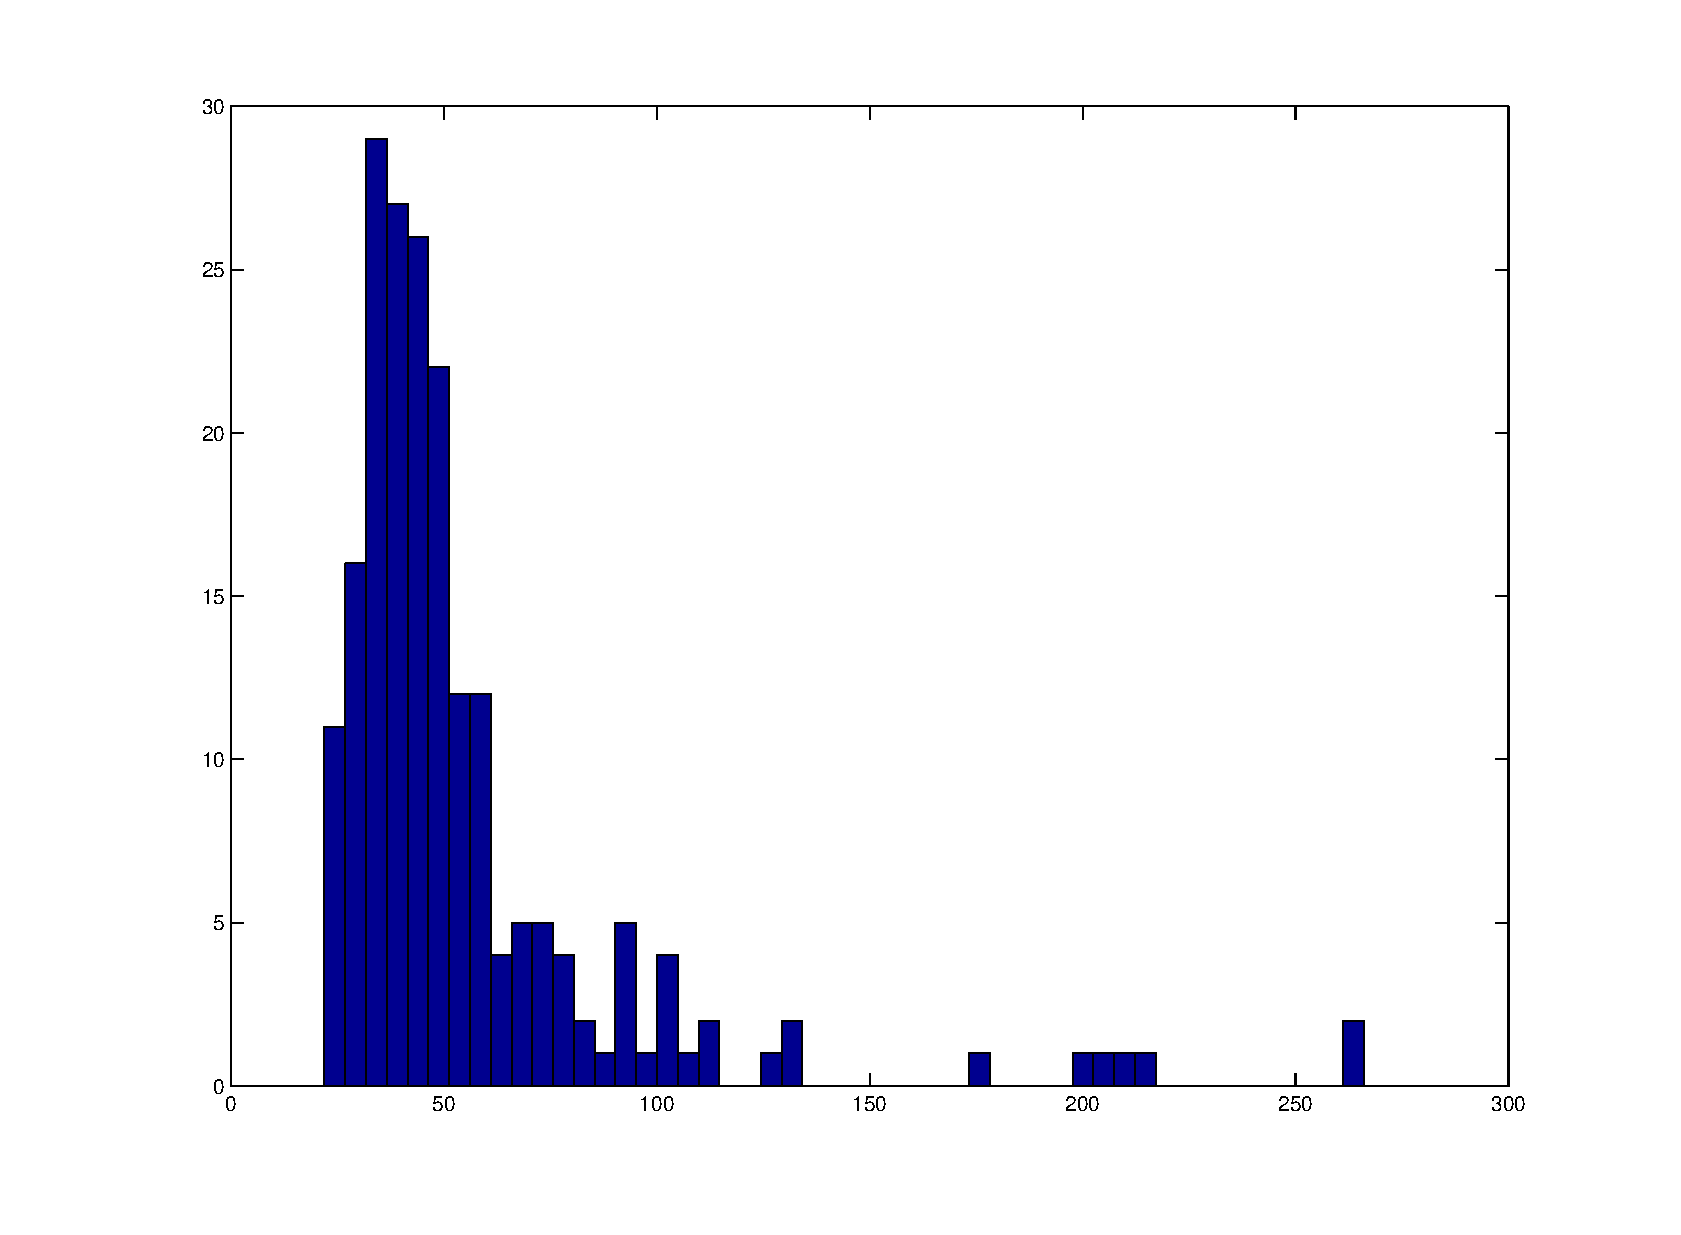
\includegraphics[scale=0.35]{histogram.eps}
\caption{Distribution of point assignments of mapper output}
\label{fig:proj3-initialisation}
\end{figure}


\subsection{Reducer}
The reducer receives for each of the 300 mappers 200 centroids-touch count pairs. We perform online K-Means on the centroids which are now viewed as weighted data in the context of the reducer.

The touch counts are considered as follows: When K-Means iterates over one point with touch count $tc_i$ it applies the centroid update step $tc_i$ times.


\bibliographystyle{plain}
\bibliography{literature}

\end{document} 
